\documentclass[9pt,aspectratio=169,xcolor=table]{beamer}

%~~~~~~~~~~~~~~~~~~~~~~~~~~~~~~~~~~~~~~~~~~~~~~~~~~~~~~~~~~~~~~~~~~~~~~~~~~~~~~
% Use roboto Font (recommended)
\usepackage[sfdefault]{roboto}
\usepackage[utf8]{inputenc}
\usepackage[T1]{fontenc}
%~~~~~~~~~~~~~~~~~~~~~~~~~~~~~~~~~~~~~~~~~~~~~~~~~~~~~~~~~~~~~~~~~~~~~~~~~~~~~~

%~~~~~~~~~~~~~~~~~~~~~~~~~~~~~~~~~~~~~~~~~~~~~~~~~~~~~~~~~~~~~~~~~~~~~~~~~~~~~~
% Define where theme files are located. ('/styles')
\usepackage{styles/fluxmacros}
\usefolder{styles}
% Use Flux theme v0.1 beta
% Available style: asphalt, blue, red, green, gray
\usetheme[style=gray]{flux}
%~~~~~~~~~~~~~~~~~~~~~~~~~~~~~~~~~~~~~~~~~~~~~~~~~~~~~~~~~~~~~~~~~~~~~~~~~~~~~~

%~~~~~~~~~~~~~~~~~~~~~~~~~~~~~~~~~~~~~~~~~~~~~~~~~~~~~~~~~~~~~~~~~~~~~~~~~~~~~~
% Extra packages
\usepackage{booktabs}
\usepackage{colortbl}
\usepackage{ragged2e}
\usepackage{amssymb}
\usepackage{multirow}
\usepackage{tikz}
\usetikzlibrary{arrows.meta, positioning, fit, backgrounds, calc, decorations.pathreplacing}
\setbeamertemplate{itemize items}[square]
\usepackage[scaled=.8]{beramono}
\usepackage{listings}
\usepackage{styles/lstlangarm}
\usepackage{array}
\definecolor{bgcolor}{HTML}{F2E9E9}
% lstlangarm.sty references \color{mauve} for string literals but never defines
% it -- only fires when a listing contains a string. Define it here.
\definecolor{mauve}{rgb}{0.58,0,0.82}
% lstlangarm's C style sets commentstyle=green!20, which is unreadable on the
% pink listing background. Darken it globally.
\lstset{commentstyle=\color{green!45!black}}
% ragged-right fixed-width column -- must be defined in the preamble, never
% inside a frame (\newcolumntype's #1 breaks beamer's frame scanner)
\newcolumntype{R}[1]{>{\RaggedRight\arraybackslash}p{#1}}
%~~~~~~~~~~~~~~~~~~~~~~~~~~~~~~~~~~~~~~~~~~~~~~~~~~~~~~~~~~~~~~~~~~~~~~~~~~~~~~
% Table striping: odd rows white, even rows very light gray.
% Needs \documentclass[...,xcolor=table]{beamer} (beamer loads xcolor itself,
% so the option must go on the class, not \usepackage).
\definecolor{stripe}{gray}{0.94}
% \striped makes body rows alternate white, gray, white, ... starting white.
% \rowcolors counts from the first coloured body row; the header is not counted.
\newcommand{\striped}{\rowcolors{1}{white}{stripe}}
%~~~~~~~~~~~~~~~~~~~~~~~~~~~~~~~~~~~~~~~~~~~~~~~~~~~~~~~~~~~~~~~~~~~~~~~~~~~~~~

%~~~~~~~~~~~~~~~~~~~~~~~~~~~~~~~~~~~~~~~~~~~~~~~~~~~~~~~~~~~~~~~~~~~~~~~~~~~~~~
% TikZ block styles -- matches ch1/ch2
% Colour variables are named identically in the book's stm32primer.tex, so any
% tikzpicture using only the \tikzset{...} styles below can be copied verbatim
% between slides and book. Only the \definecolor/\colorlet VALUES differ: the
% book is printed, so it keeps every stroke pure black with muted fills. These
% slides are projected, so both fill AND stroke are bright and saturated to
% grab attention -- see stm32primer.tex for the print palette.
\definecolor{blkfill}{HTML}{DCEBFF}
\definecolor{blkline}{HTML}{1565C0}
\definecolor{accentfill}{HTML}{FFE0B2}
\definecolor{accentline}{HTML}{E65100}
\definecolor{memfill}{HTML}{DFF5DA}
\definecolor{memline}{HTML}{2E7D32}
\definecolor{cellfill}{HTML}{FFFFFF}
\definecolor{cellline}{HTML}{424242}
\definecolor{bitmaskfill}{HTML}{DCEBFF}
\definecolor{bitmaskline}{HTML}{1565C0}
\definecolor{bithitfill}{HTML}{FFE0B2}
\definecolor{bithitline}{HTML}{E65100}
\tikzset{
  blk/.style   = {rectangle, rounded corners=2pt, draw=blkline, fill=blkfill,
                  thick, align=center, font=\small, minimum height=9mm, inner sep=3pt},
  cpublk/.style= {rectangle, rounded corners=2pt, draw=accentline, fill=accentfill,
                  thick, align=center, font=\small\bfseries, minimum height=9mm, inner sep=3pt},
  memblk/.style= {rectangle, rounded corners=2pt, draw=memline, fill=memfill,
                  thick, align=center, font=\small, minimum height=9mm, inner sep=3pt},
  cell/.style  = {rectangle, draw=cellline, fill=cellfill, align=center,
                  font=\small\ttfamily, minimum height=7mm, inner sep=2pt},
  lbl/.style   = {font=\scriptsize, text=Gray},
  flow/.style  = {-{Stealth[length=2mm]}, thick, draw=blkline},
  busline/.style={thick, draw=cellline},
}
% NOTE (theme quirks -- all fail SILENTLY, always page through the PDF):
%  - a second \\ inside a nested {...} group in a TikZ node breaks parsing
%  - {\small ...} wrapped around a nested itemize eats the frame title + list
%  - \usebeamercolor on a [plain] frame falls through to an unstyled default
%  - \newcolumntype inside a frame breaks beamer's frame scanner
%  - lstlisting needs \begin{frame}[fragile]
%  - a TikZ picture wider than its column silently overflows into neighbours
%~~~~~~~~~~~~~~~~~~~~~~~~~~~~~~~~~~~~~~~~~~~~~~~~~~~~~~~~~~~~~~~~~~~~~~~~~~~~~~

%%%%%%%%%%%%%%%%%%%%%%%%%%%%%%%%%%%
%% BEGIN CONDITIONAL COMPILATION %%
%%%%%%%%%%%%%%%%%%%%%%%%%%%%%%%%%%%
\newif\ifwebex
%\webextrue % uncomment to generate section separator
\ifwebex
\AtBeginSection[]{
  \begin{frame}
  \vfill
  \centering
  \begin{beamercolorbox}[sep=8pt,center,shadow=true,rounded=true]{title}
    \usebeamerfont{title}\insertsectionhead\par%
  \end{beamercolorbox}
  \vfill
  \end{frame}
}
\else
\AtBeginSection[]
{
{
    \setbeamercolor{background canvas}{bg=yellow!10}
    \begin{frame}[plain]
        \frametitle{Table of Contents}
        \tableofcontents[currentsection]
    \end{frame}
}
}
\fi
%%%%%%%%%%%%%%%%%%%%%%%%%%%%%%%%%%%
%% END CONDITIONAL COMPILATION   %%
%%%%%%%%%%%%%%%%%%%%%%%%%%%%%%%%%%%

%~~~~~~~~~~~~~~~~~~~~~~~~~~~~~~~~~~~~~~~~~~~~~~~~~~~~~~~~~~~~~~~~~~~~~~~~~~~~~~
% Information
\title{Designing, Building and Verifying an Embedded System}
\subtitle{\emph{Introduction to ARM Cortex-M Microprocessors} --- Chapter 14}
\author{Mun\'{i}m Zabidi}
\institute{\color{primary}Faculty of Electrical Engineering, Universiti Teknologi Malaysia}
\date{\today}
\titlegraphic{assets/logoutmwhite.png}
%~~~~~~~~~~~~~~~~~~~~~~~~~~~~~~~~~~~~~~~~~~~~~~~~~~~~~~~~~~~~~~~~~~~~~~~~~~~~~~

\begin{document}

\titlepage

\begin{frame}{Table of Contents}
    \tableofcontents
\end{frame}

%===============================================================================
\section{Why This Matters}
%===============================================================================

\begin{frame}{Why This Chapter Matters}
    \leavevmode
    Every previous chapter examined one peripheral in isolation. Real systems are not like that: they sample on a schedule while responding to buttons, driving indicators, and reporting to a host --- all at once, on one processor, with no operating system. But the hard part is neither the peripherals nor the code. It is deciding, before any code exists, which peripherals the requirement demands and whether the timing can be met at all --- and then \emph{showing} that the result meets the requirement rather than merely appearing to work. This chapter does all three, in the order an engineer works in.
\end{frame}

\begin{frame}{Objectives}
    \leavevmode
    {\small After completing this chapter, you should be able to:}

    \vspace{2mm}
    {\small
    \begin{enumerate}\itemsep2pt
        \item Turn a written requirement into a functional decomposition and a peripheral selection.
        \item Choose between polling, timed polling, and interrupt-driven structures for a given activity.
        \item Structure a bare-metal program using a non-blocking cooperative main loop.
        \item Identify and protect shared data between interrupt and main contexts.
        \item Produce a timing budget before implementation and verify it by measurement afterwards.
        \item Apply a systematic bottom-up procedure to diagnose a multi-peripheral system.
    \end{enumerate}}
\end{frame}


%===============================================================================
\section{From Requirement to Architecture}
%===============================================================================

\begin{frame}{The Step Before Any Code}
    \leavevmode
    A requirement is prose. An architecture is a set of decisions. Getting from
    one to the other is \alert{the engineering}, and it happens on paper.

    \vspace{3mm}
    \begin{center}
    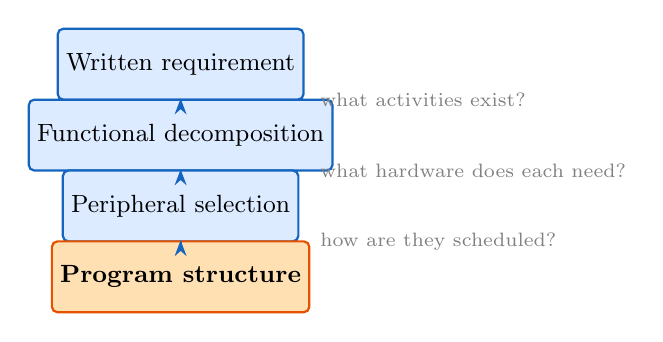
\begin{tikzpicture}[x=10mm, y=9mm]
        \node[blk,    minimum width=28mm] (r) at (0,1.5)  {Written requirement};
        \node[blk,    minimum width=28mm] (f) at (0,0.5)  {Functional decomposition};
        \node[blk,    minimum width=28mm] (p) at (0,-0.5) {Peripheral selection};
        \node[cpublk, minimum width=28mm] (s) at (0,-1.5) {Program structure};
        \foreach \x/\y in {r/f, f/p, p/s}{\draw[flow] (\x) -- (\y);}
        \node[lbl, anchor=west] at (1.65,1.0)  {what activities exist?};
        \node[lbl, anchor=west] at (1.65,0.0)  {what hardware does each need?};
        \node[lbl, anchor=west] at (1.65,-1.0) {how are they scheduled?};
    \end{tikzpicture}
    \end{center}

    \vspace{2mm}
    \begin{block}{Why this order matters}
        Choosing peripherals before decomposing the activities means you discover
        the pin conflict \alert{after} the board is made.
    \end{block}
\end{frame}

\begin{frame}{Four Ways to Structure an Activity}
    \begin{center}
    {\small
    \striped
    \begin{tabular}{@{}l R{.34\textwidth} R{.32\textwidth}@{}}
        \toprule
        \textbf{Structure} & \textbf{Use when} & \textbf{Cost} \\
        \midrule
        \textbf{Blocking poll} & Never, in a real system & Burns the CPU; blocks everything else \\
        \textbf{Timed poll} & The activity has a known period and loose jitter & Simple; jitter is the loop time \\
        \textbf{Interrupt} & The event is external and the deadline is tight & Needs care with shared data \\
        \textbf{DMA} & Bulk data, no per-byte decision & Setup cost; fewest CPU cycles \\
        \bottomrule
    \end{tabular}}
    \end{center}

    \vspace{3mm}
    \begin{block}{The decision is per activity, not per program}
        One system routinely uses all four: DMA for an ADC stream, an interrupt
        for a button, a timed poll for a display refresh, and the main loop for
        everything with no deadline at all.
    \end{block}
\end{frame}

%===============================================================================
\section{The Non-Blocking Main Loop}
%===============================================================================

\begin{frame}[fragile]{The Pattern}
\begin{lstlisting}[language=C, basicstyle=\ttfamily\scriptsize]
while (1) {
    uint32_t now = millis();

    if (now - last_sensor >= 2000) {    // every 2 s
        last_sensor = now;
        read_sensor();
    }
    if (now - last_display >= 100) {    // every 100 ms
        last_display = now;
        update_display();
    }
    if (button_flag) {                  // set by an ISR
        button_flag = 0;
        handle_button();
    }
}
\end{lstlisting}

    \vspace{2mm}
    \begin{block}{Nothing waits}
        Each activity asks ``is it my turn yet?'' and returns immediately if not.
        The loop runs thousands of times per second, and every activity gets
        serviced \alert{close enough} to its deadline.
    \end{block}
\end{frame}

\begin{frame}{Why \texttt{now - last >= period} and Not \texttt{now >= next}}
    \begin{columns}[T]
    \begin{column}{.48\textwidth}
        \textbf{The subtraction form}

        \vspace{1mm}
        {\ttfamily\scriptsize if (now - last >= 2000)}

        \vspace{2mm}
        {\small Survives the 32-bit counter \alert{wrapping} after 49 days,
        because unsigned subtraction wraps consistently.}
    \end{column}
    \begin{column}{.48\textwidth}
        \textbf{The comparison form}

        \vspace{1mm}
        {\ttfamily\scriptsize if (now >= next)}

        \vspace{2mm}
        {\small \alert{Breaks} at the wrap: \texttt{next} is a huge number,
        \texttt{now} has reset to a small one, and the activity stops for
        49 days.}
    \end{column}
    \end{columns}

    \vspace{3mm}
    \begin{block}{A bug you cannot find by testing}
        It appears once, after seven weeks of continuous running. This is exactly
        the class of fault that \alert{reasoning} catches and \alert{testing} does
        not --- which is why the argument matters more than the code.
    \end{block}
\end{frame}

\begin{frame}{Sharing Data With an ISR}
    \begin{columns}[T]
    \begin{column}{.48\textwidth}
        \textbf{Two hazards}
        {\small
        \begin{itemize}\itemsep1pt
            \item \alert{Missing \texttt{volatile}} --- the optimiser caches a
                  value the ISR changes
            \item \alert{Torn access} --- \texttt{main()} reads a multi-word
                  variable while the ISR is halfway through writing it
        \end{itemize}}
    \end{column}
    \begin{column}{.48\textwidth}
        \textbf{Three defences}
        {\small
        \begin{itemize}\itemsep1pt
            \item Mark it \texttt{volatile}
            \item Keep it to a single \texttt{uint32\_t} --- read atomically on a
                  32-bit machine
            \item Or disable interrupts \alert{briefly} around the access
        \end{itemize}}
    \end{column}
    \end{columns}

    \vspace{3mm}
    \begin{block}{The flag pattern}
        The ISR does the minimum --- clear the hardware flag, set a software one,
        return. \texttt{main()} does the real work. That keeps the handler short
        \alert{and} keeps the shared state to one byte.
    \end{block}
\end{frame}

%===============================================================================
\section{Verification}
%===============================================================================

\begin{frame}{The Timing Budget}
    \leavevmode
    Write it \alert{before} implementation, and it tells you whether the design is
    possible at all.

    \vspace{3mm}
    \begin{center}
    {\small
    \striped
    \begin{tabular}{@{}l l l l@{}}
        \toprule
        \textbf{Activity} & \textbf{Period} & \textbf{Duration} & \textbf{Load} \\
        \midrule
        SysTick ISR      & 1\,ms   & 2\,\textmu s   & 0.2\,\% \\
        Sensor read      & 2\,s    & 400\,\textmu s & 0.02\,\% \\
        Display update   & 100\,ms & 3\,ms          & 3\,\% \\
        Button ISR       & rare    & 5\,\textmu s   & $\approx 0$ \\
        \midrule
        \textbf{Total}   &         &                & \alert{$\approx 3.3\,\%$} \\
        \bottomrule
    \end{tabular}}
    \end{center}

    \vspace{3mm}
    \begin{block}{What the number tells you}
        3\,\% means comfortable headroom. \alert{80\,\% means the design is
        fragile} --- one slow path and a deadline is missed. Over 100\,\% means it
        cannot work, and you know that before writing a line.
    \end{block}
\end{frame}

\begin{frame}{Predict, Then Measure}
    \begin{columns}[T]
    \begin{column}{.48\textwidth}
        \textbf{The discipline}
        \begin{enumerate}
            \item \alert{Predict} the number --- period, duty cycle, execution
                  time
            \item \alert{Measure} it
            \item When they disagree, \alert{find out why}
        \end{enumerate}
    \end{column}
    \begin{column}{.48\textwidth}
        \textbf{How to measure}
        {\small
        \begin{itemize}\itemsep1pt
            \item Set a GPIO pin high on entry, low on exit --- watch it on a
                  scope
            \item Read \texttt{SysTick->VAL} before and after
            \item Toggle a pin per loop iteration and measure the frequency
        \end{itemize}}
    \end{column}
    \end{columns}

    \vspace{3mm}
    \begin{block}{The disagreement is the finding}
        If you predicted 400\,\textmu s and measure 3\,ms, you have learned
        something --- about the compiler, the clock tree, or your own assumptions.

        \vspace{1mm}
        \alert{Measuring without predicting teaches you nothing}, because any
        number looks plausible.
    \end{block}
\end{frame}

\begin{frame}{What a Working Demonstration Does Not Prove}
    \begin{columns}[T]
    \begin{column}{.5\textwidth}
        \textbf{It runs. What is still unknown?}
        {\small
        \begin{itemize}\itemsep1pt
            \item Whether it survives the \alert{counter wrap} at 49 days
            \item Whether the deadline is met in the \alert{worst case}, not the
                  typical one
            \item Whether a shared variable is ever \alert{torn}
            \item What happens when a sensor \alert{fails} rather than reads wrong
            \item Whether it works at the \alert{temperature extremes}
        \end{itemize}}
    \end{column}
    \begin{column}{.46\textwidth}
        \begin{block}{Demonstration is evidence, not proof}
            A demo shows the system works \alert{once, here, now}, under the
            conditions you happened to create.

            \vspace{2mm}
            Everything else you believe about it comes from \alert{argument}: the
            timing budget, the wrap analysis, the reasoning about shared state.
        \end{block}
    \end{column}
    \end{columns}
\end{frame}

\begin{frame}{A Debugging Methodology}
    \leavevmode
    When a multi-peripheral system misbehaves, work \alert{bottom-up}. Each step
    either finds the fault or eliminates a layer.

    \vspace{1mm}
    \begin{center}
    {\small
    \striped
    \begin{tabular}{@{}l R{.60\textwidth}@{}}
        \toprule
        \textbf{Step} & \textbf{Question} \\
        \midrule
        1 & Is the \alert{clock} enabled for this peripheral? \\
        2 & Is the \alert{pin} in the right mode, with the right alternate function? \\
        3 & Does the \alert{register} read back what you wrote? \\
        4 & Does the peripheral's \alert{status flag} ever set? \\
        5 & Does the \alert{ISR} run --- toggle a pin inside it and look \\
        6 & Is the \alert{shared variable} \texttt{volatile}, and read atomically? \\
        7 & Does the \alert{timing} match the budget you predicted? \\
        \bottomrule
    \end{tabular}}
    \end{center}

    \vspace{1mm}
    {\small Steps 1 and 2 account for most first-time faults --- and
    \alert{a register that does not read back is an unclocked peripheral}.}
\end{frame}

\begin{frame}{What You Have Learned}
    \begin{columns}[T]
    \begin{column}{.48\textwidth}
        \textbf{The mechanism}
        {\small
        \begin{itemize}\itemsep1pt
            \item A CPU fetches, decodes, executes --- forever
            \item Memory is numbered; some numbers are hardware
            \item C reaches them through \alert{pointers}
            \item Instructions are what your C becomes
        \end{itemize}}
    \end{column}
    \begin{column}{.48\textwidth}
        \textbf{The practice}
        {\small
        \begin{itemize}\itemsep1pt
            \item Enable the clock first
            \item \texttt{volatile} on everything hardware touches
            \item Read--modify--write preserves the neighbours
            \item Interrupts for deadlines, timers for time
            \item \alert{Predict, then measure}
        \end{itemize}}
    \end{column}
    \end{columns}

    \vspace{3mm}
    \begin{block}{The one sentence from Chapter 1}
        \alert{The CPU has no special instruction for ``turn on an LED''.} It has
        instructions that read and write addresses --- and some of those addresses
        are wired to hardware.

        \vspace{1mm}
        Everything in the thirteen chapters since has been an elaboration of that.
    \end{block}
\end{frame}

%===============================================================================
\section{Design Challenge}
%===============================================================================

\begin{frame}{Design Challenge}{To be worked on paper, before any code}
    \leavevmode
    \begin{block}{The brief}
        A greenhouse controller must: read a temperature sensor every 2~s; read a soil-moisture sensor every 30~s; drive a ventilation fan through a PWM output whose duty follows temperature; open a water valve (a single digital output) for 5~s whenever moisture falls below a threshold; accept a manual override button at any time; and report all readings to a host once per minute.
    \end{block}

    \vspace{2mm}
    {\small Do not write any code. Produce the design: the functional decomposition, the peripheral assigned to each activity, the event structure chosen for each (with justification), a pin allocation checked for collisions on the STM32F446RE, a timing budget, and the initialization order. Then write the verification plan that would accompany it: what measurement establishes each timing requirement, with what instrument, and what the acceptance criterion is. Identify the one activity whose timing is hardest to guarantee, and the single measurement you would take first.}
\end{frame}

\begin{frame}[plain]
    \begin{center}
        \vfill
        {\usebeamerfont{title}\color{primary}\Huge Questions?}
        \vfill
        {\small\color{Gray} \emph{Introduction to ARM Cortex-M Microprocessors} --- Chapter 14}
        \vfill
    \end{center}
\end{frame}

\end{document}

